\chapter{03 Forelesning Notater}
\section{Sentrale Kunnskaper}
\begin{itemize}
    \item Beskrive den fotoelektriske effekten og 
    \item Hvordan Einsteins teori forklarer de tre ekps. observasjonene. Forstå hva det betyr at et materialet har arbeidsfunksjon $w_0$. Håndtere og beregne $K_{\text{max}} = hν - w_0$
    \item Beskrive hvordan Röntgen-stråling-eksp. støtter Einsteins teori.
\end{itemize}
\section{Fotoelektrisk Effekt}


\begin{figure}[h!]
  \centering
  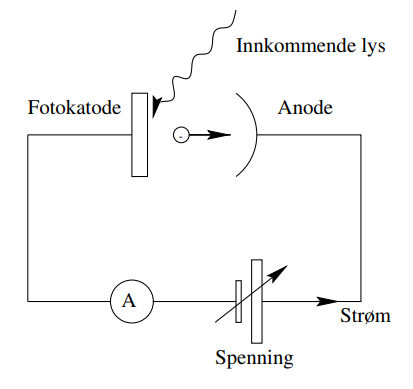
\includegraphics[scale = .5]{Figures/Fotoeletkrisk effekt oppsett.png}
  \caption{Oppsett av den fotoelektriske effekten}
  \label{fig: Fotoelektrisk effekt oppsett}
\end{figure}
Spenningen $V$ fra Anoden til Fotokatoden skaper et elektrisk felt fra Anoden til Fotokatoden. Her går det ikke noe strøm. Hvis vi sender elektromagnetisk stråling på Fotokatoden får vi en fotostrøm strøm gjennom kretsen. Dette må bety at strålingen frigjør elektroner i materialet.

Intensiteten til lyset definers som $I = \frac{E}{As}$ hvor $E$ er energi, $s$ er tid og $A$ er areal. Intensitet måles i $W / m^{2}$

Den kinetiske energien $K$ til et elektron er definert ved overflaten til materialet til Fotokatoden. 

Det elektriske feltet vil akselererer elektronene som fører til en økning i kinetisk energi gitt ved 
\[
K + eV. 
\]
Illustrert i figur \ref{fig: Fotoelektrisk effekt oppsett}, har vi en positiv spenning ved Anoden. Hvis vi snur dette til en negativ spenning $-V$. Da vil elektronene ha en kinetisk energi $K_{\text{overflate}}$, som motvirkes av det elektriske feltet. Elektronene vil da gå tilbake til materialet. Hvis den kinetiske energien er høy nok kan elektronene nå frem til Anoden i andre enden. Da blir den kinetiske energien $K = K_{\text{overflate}} - \left\vert eV \right\vert $. Da må naturligvis $K_{\text{overlfate}} \ge  eV$. 

Dette fenomenet ble avdekket tre observasjoner. 

\subsection{Observasjon 1}
For å undersøke strømmen som funksjon av spenningen setter vi en konstant intensitet og frekvens på lyset. Når vi minker spenningen vil strømmen også minke ettersom elektronene krever mer kinetisk energi for å nå Anoden. Til slutt vil strømmen ta fullstendig slutt når vi setter på en spenning $-V_0$. Ved denne spenningen er $K < \left\vert eV_0 \right\vert $. Vi setter da $K_{\text{maks}} = \left\vert eV_0 \right\vert $. Strømmen med dette oppsette er notert ved $I_1$ sett i figur \ref{fig: Fotoelektrisk resultat}

\begin{figure}[h!]
  \centering
  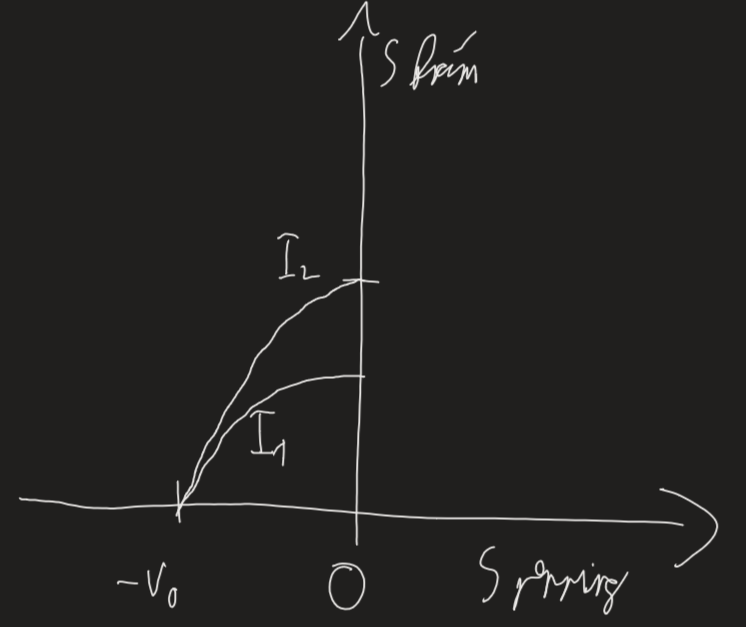
\includegraphics[scale = .4]{Figures/Fotoelektrisk resultat.png}
  \caption{Eksperimentelle resultater av fotoelektrisk effekt}
  \label{fig: Fotoelektrisk resultat}
\end{figure}


Nå kommer det som kræsjer med klassisk fysikk. Hvis vi øker intensiteten på strålingen forventer vi at elektronene får høyere kinetisk energi, og flere elektroner blir en del av fotostrømmen. Det stemmer at en får mer strøm $I_2$, men strømmen stopper ved samme spenning $-V_0$ som sett i figur \ref{fig: Fotoelektrisk resultat}. 

\subsection{Observasjon 2}
Neste forsøk som sett i figur \ref{fig: Fotoelektrisk resultat 2} valgte man å holde intensitet konstant og varierer spenningen $ν$. Da ser man at max kinetisk energi øker lineært med frekvensen på lyset. $K_{\text{max}}$ går mot null når frekvensen går mot $ν_0 > 0$. Frekvensen dikterer hva som er den maksimale kinetiske energien til elektronene, og dermed størrelsen på spenningen $V_0$ som sett i figur \ref{fig: fotoelektrisk resultat 2.1}.
\begin{figure}[h!]
  \centering
  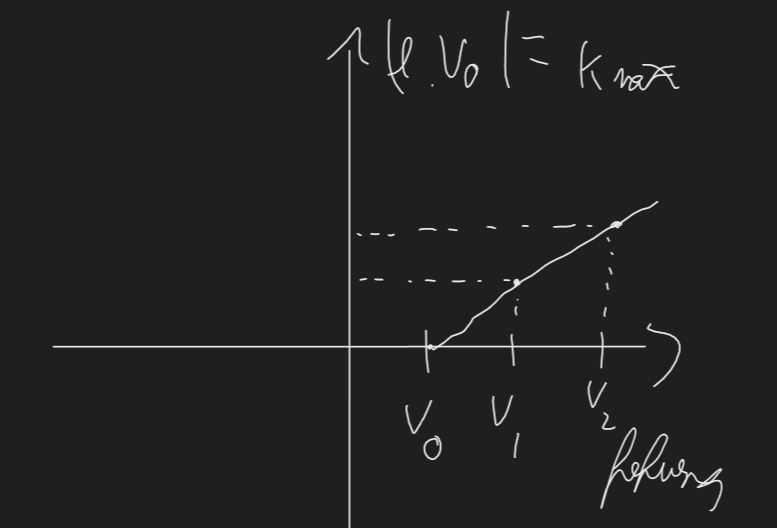
\includegraphics[scale = .4]{Figures/Fotoelektrisk resultat 2.png}
  \caption{Eksperimentelle resultater av fotoelektrisk effekt med varierende frekvens $ν$}
  \label{fig: Fotoelektrisk resultat 2}
\end{figure}

\begin{figure}[h!]
    \centering
    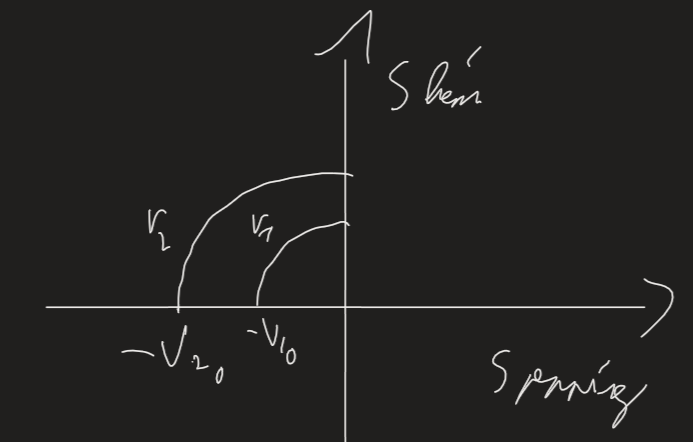
\includegraphics[scale = .4]{Figures/fotoelektrisk resultat 2.1.png}
    \caption{Strøm som en funksjon av spenning}
    \label{fig: fotoelektrisk resultat 2.1}
  \end{figure}


\subsection{Observasjon 3}
En la merke til at fotostrømmen skjer nesten øyeblikkelig. Det betyr at det elektronene ikke krever mye tid for å få en kinetisk energi $K = \left\vert eV_0 \right\vert $. Dette er uavhengig av intensiteten på strålingen.

\subsubsection{Oppsummert}
  1a. Det eksisterer en stoppepotensial $V_0$, og ingen elektroner har $K \ge  \left\vert eV_0 \right\vert $. 
  
  1b. $K_{\text{maks}} = \left\vert e V_0 \right\vert $ uavhengig av intensiteten på strålingen.
  
  2a. $K_{\text{maks}}$ øker lineært med frekvensen på strålingen.
  
  2b. $K_{\text{maks}}$ går mot null når frekvensen går mot $ν_0 > 0$
  
  3. Fotostrømmen skjer nesten øyeblikkelig.

\subsubsection{Einsteins Forklaring}
Einstein så på lyset som små energi pakker i stedet for et kontinuerlig bølgefelt. Hvert foton vil da ha en energi $E = hν$. Fotonene vil frigjøre elektronene i materialet. Dette vil da gi elektronene en energi $E = hν$, som kan være nok til å komme på utsiden av materialet. Det krever litt energi så elektronet vil ha en kinetisk energi $K = hν - ω$, der $ω$ er energien tapt på vei til overflaten. Da vil $K_{\text{maks}} = hν - ω_0$ ettersom $ω_0$ er den minste energien som kreves for å løsrive det svakest bunnende elektronet. $ω_0$ er arbeidsfunksjonen. 

Dette er i et ideelt tilfelle hvor elektronene ikke kolliderer med hverandre eller går i andre retninger enn rett mot Anoden. Det viktigste å få med seg er hvordan Einstein forklarer at $K_{\text{maks}}$ er uavhengig av intensiteten på strålingen, bare frekvensen. 


\section{Röntgen-Stråling}

\begin{figure}[h!]
    \centering
    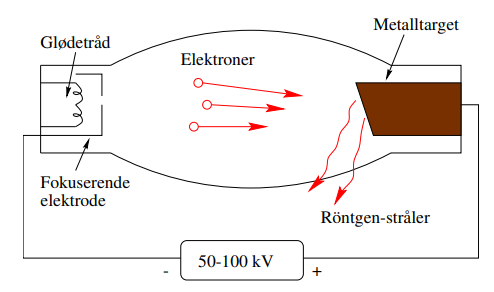
\includegraphics[scale = .5]{Figures/Rontgenstraaling oppsett.png}
    \caption{Oppsett av röntgenstråling eksperimentet}
    \label{fig: Rontgenstraaling oppsett}
\end{figure}

\begin{figure}[h!]
  \centering
  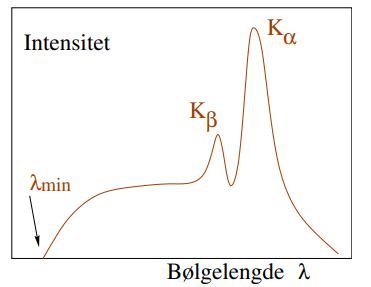
\includegraphics[scale = .5]{Figures/Rontgenstraaling intensitetfordeling.png}
  \caption{Intensitet fordeling ved Röntgenstråling}
  \label{fig: Intensitets fordeling Rontgenstraaling}
\end{figure}

Dette er det motsatte av fotoelektrisk effekt. Her skytes elektroner på et materialet som skyter ut fotoner. Den maksimale energien et utstrålt foton kan ha er gitt ved 
\[
E_{\text{maks}} = \frac{hc}{\lambda} = hν
\]

  